% =====================================================================
% FISCAL-CONTEXT FIGURES  --  drop-in snippet
% Figures produced by code/fiscal_context_figures.R (set WRITE_FIGURES <- TRUE).
% PDFs land in paper/Figures/.
% =====================================================================

% ---------------------------------------------------------------------
% (A) MAIN TEXT  --  paste into Section~\ref{sec:institutional}
%     (Institutional Background), right after the paragraph ending
%     "...between 17 and 33 percent of total tax revenue \parencite{nso_government_budget}."
% ---------------------------------------------------------------------

Figure~\ref{fig:vat_tax_share} sets the reform in its fiscal context. VAT is
the second-largest tax after income taxes: over 2005--2024 it supplied between
18 and 31 percent of total tax revenue and 4.6 to 8.5 percent of GDP
\parencite{nso_government_budget, nso_gdp}. Both ratios reached a local trough
around the reform---VAT raised only 20.5 percent of tax revenue in 2015 and
4.6 percent of GDP---and then recovered over the following years as the
economy expanded and ebarimt coverage widened. Overall tax revenue relative
to GDP fell to 20.7 percent in 2016, its lowest in the period, before rising
to 34 percent by 2024. Real VAT collections, deflated by the CPI, follow the
same path: a decline through 2014--2015 and a sustained increase afterwards,
close to tripling in constant terms between 2015 and 2024 (Appendix
Figure~\ref{fig:fiscal_ratios_panel}). These aggregates are descriptive---
commodity prices, import volumes, and the 2020 pandemic all move them---but
their timing around 2016 is consistent with the firm-level compliance channel
this thesis isolates. 

\begin{figure}[H]
    \centering
    \caption{\textbf{VAT's Share of Mongolian Tax Revenue, 2005--2024}}
    \label{fig:vat_tax_share}
    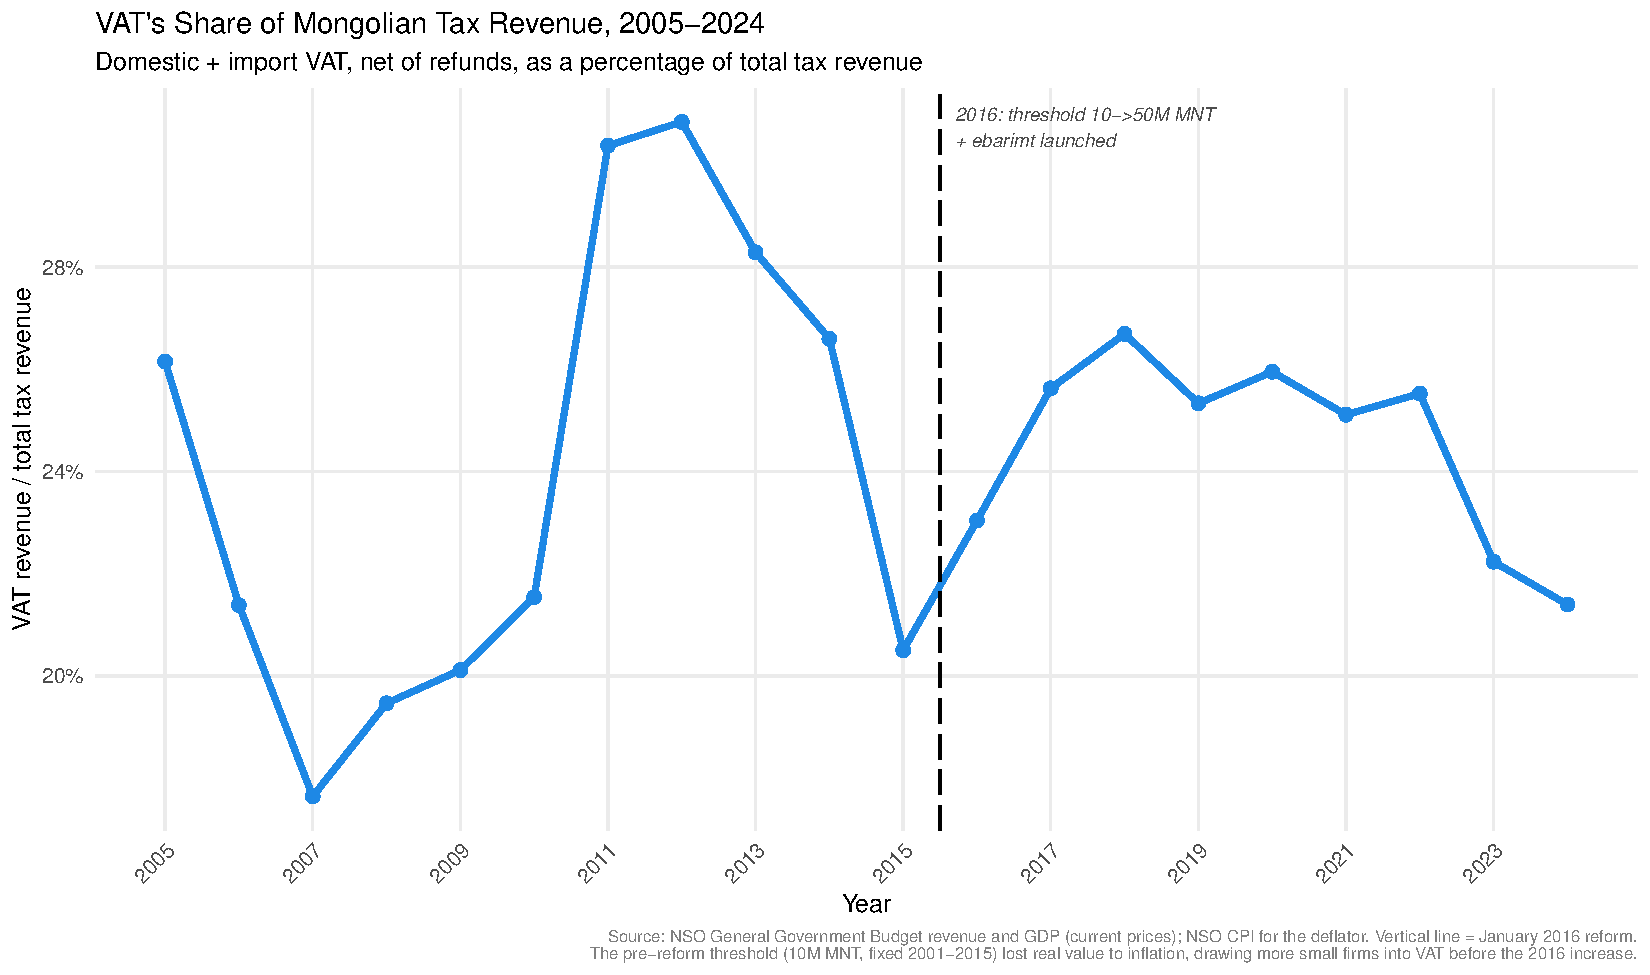
\includegraphics[width=\textwidth]{Figures/fig_vat_tax_share.pdf}
    \vspace{0.5em}
    \\ \footnotesize
    \begin{minipage}{0.92\textwidth}
    \small\textit{Notes:} Value-added tax (domestic plus import VAT, net of
    refunds) as a percentage of total tax revenue. The vertical dashed line
    marks the January 2016 reform (registration threshold 10M~$\rightarrow$~50M
    MNT and the launch of ebarimt). \textit{Source:} NSO General Government
    Budget revenue \parencite{nso_government_budget}.
    \end{minipage}
\end{figure}


% ---------------------------------------------------------------------
% (B) APPENDIX  --  paste into the appendix
% ---------------------------------------------------------------------

\begin{figure}[H]
    \centering
    \caption{\textbf{Mongolia: VAT and the Fiscal Aggregates Around the 2016 Reform}}
    \label{fig:fiscal_ratios_panel}
    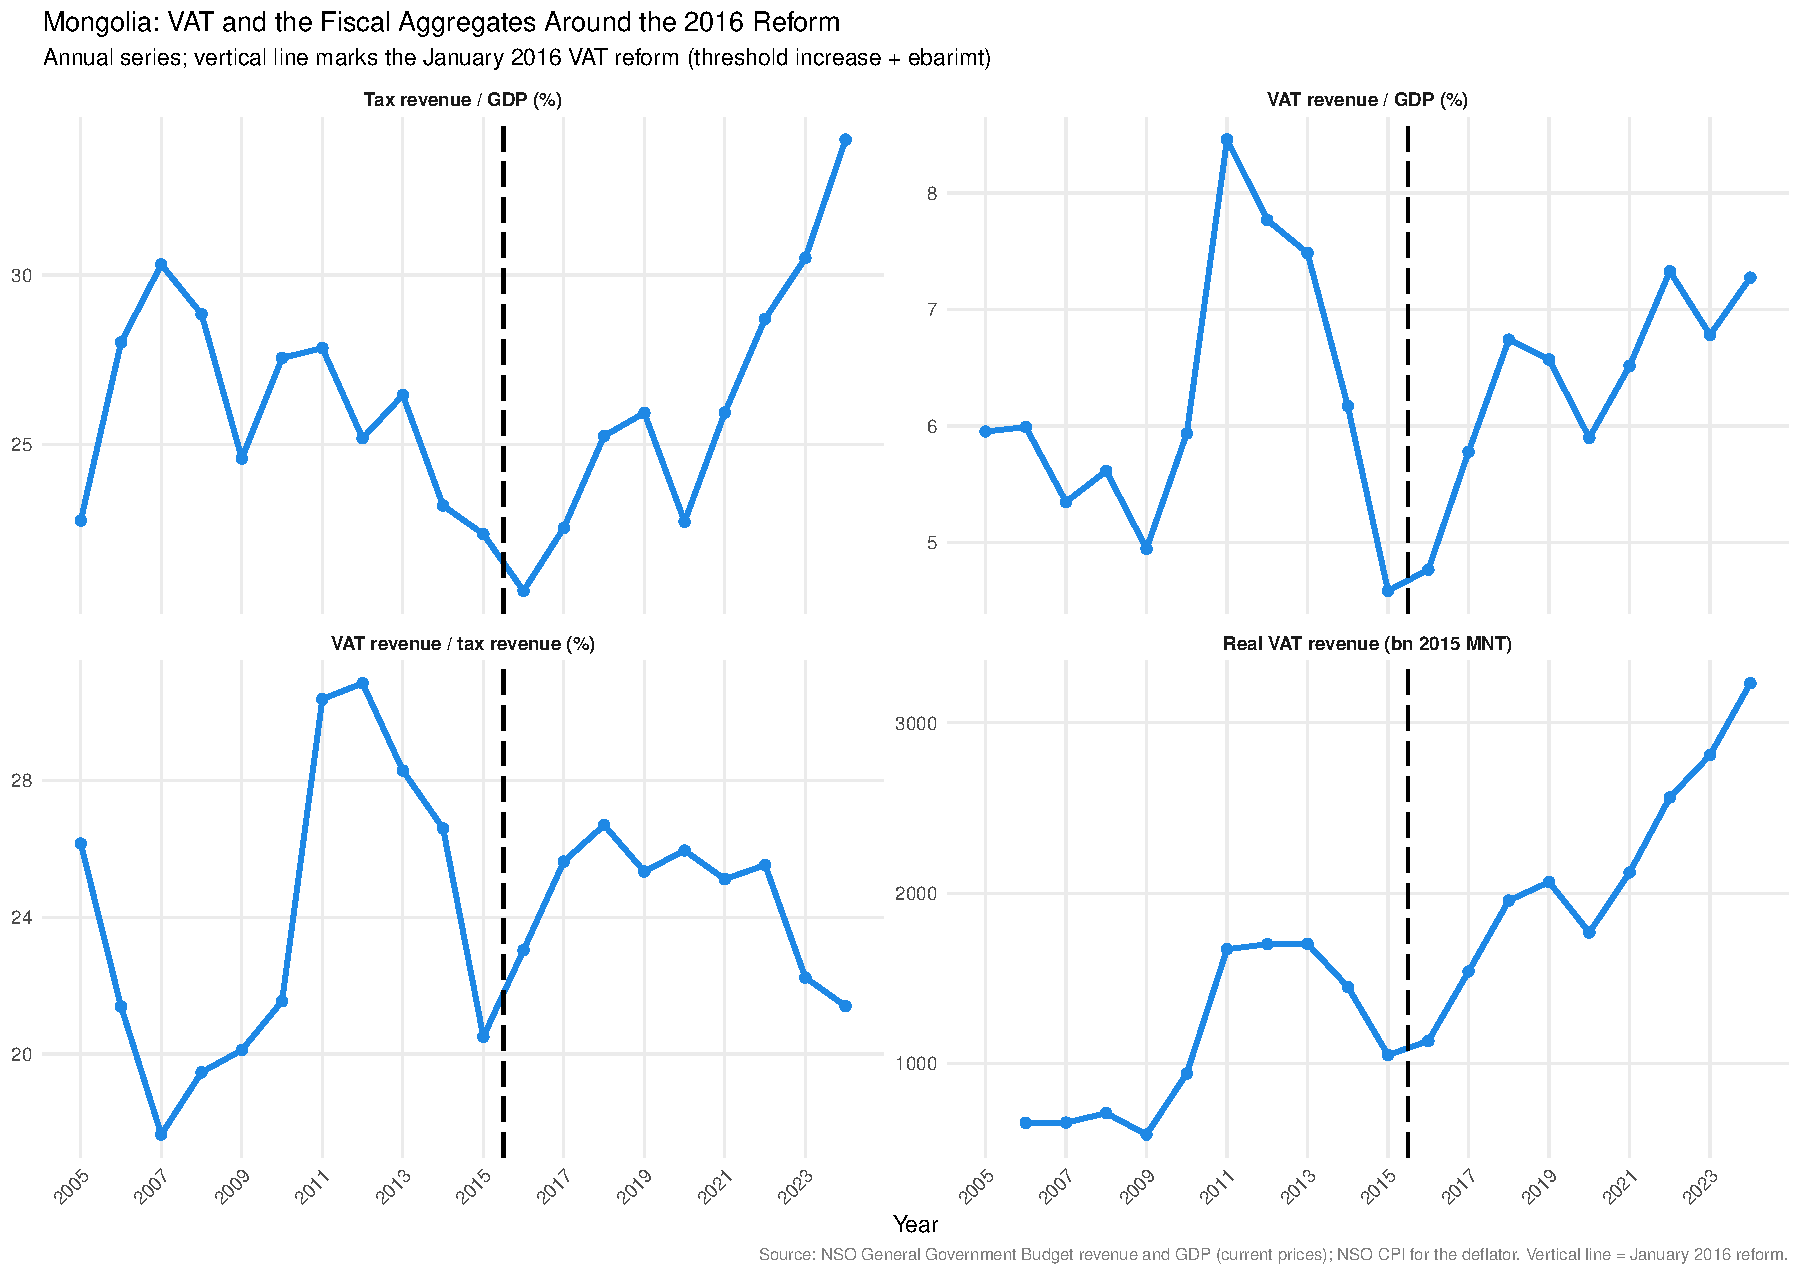
\includegraphics[width=\textwidth]{Figures/fig_fiscal_ratios_panel.pdf}
    \vspace{0.5em}
    \\ \footnotesize
    \begin{minipage}{0.92\textwidth}
    \small\textit{Notes:} Annual series. \textit{Tax revenue / GDP} and
    \textit{VAT revenue / GDP} use GDP at current prices; \textit{VAT revenue /
    tax revenue} is VAT as a share of total tax revenue; \textit{Real VAT
    revenue} is nominal VAT deflated by the CPI (annual average, spliced across
    the 2015=100 and 2020=100 base years), in billions of constant 2015 MNT.
    The vertical dashed line marks the January 2016 reform. 2025 is omitted as
    preliminary. \textit{Source:} NSO General Government Budget revenue
    \parencite{nso_government_budget}, NSO GDP \parencite{nso_gdp}, and NSO CPI.
    \end{minipage}
\end{figure}


% ---------------------------------------------------------------------
% (C) references.bib  --  add if these keys are not already defined
% ---------------------------------------------------------------------
%
% @misc{nso_gdp,
%   author       = {{National Statistics Office of Mongolia}},
%   title        = {Gross Domestic Product, by Production Approach (Current Prices)},
%   howpublished = {Statistical database, \url{https://www.1212.mn}},
%   year         = {2025}
% }
%
% @misc{nso_cpi,
%   author       = {{National Statistics Office of Mongolia}},
%   title        = {Consumer Price Index},
%   howpublished = {Statistical database, \url{https://www.1212.mn}},
%   year         = {2025}
% }
